\label{sec:daq}

The HPS experiment data acquisition (DAQ) handles the acquisition of data and for the three sub-detectors: the SVT, ECal and the Muon System. HPS employs two DAQ architectures: the SVT is readout with 
Advanced Telecom Communications Architecture (ATCA) hardware
while the ECal and Muon system use VXS based hardware. The trigger system receives input from the 
ECal and Muon System, and distributes a trigger signal to all three detector sub-systems to readout a selected  event. Figure~\ref{fig:daq_hardware_overview} gives a schematic block diagram of the DAQ system.


\begin{figure*}[ht]
%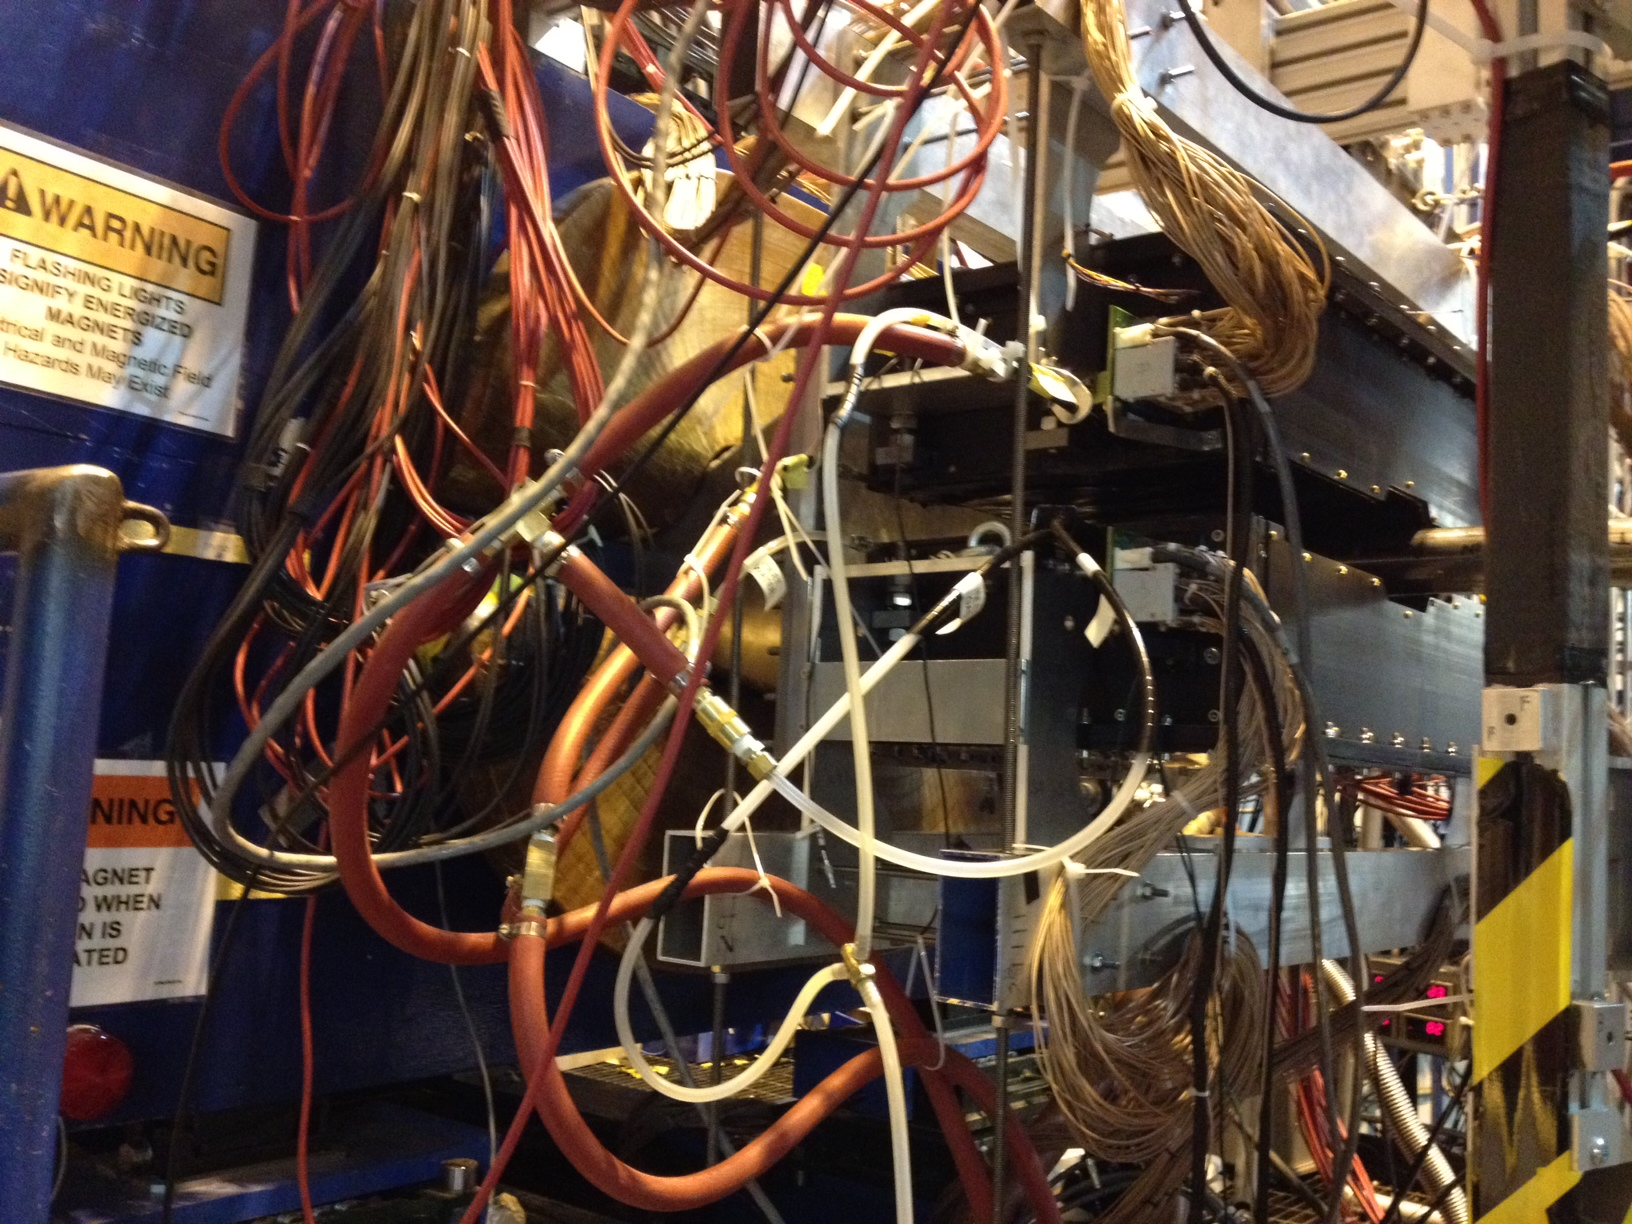
\includegraphics[ scale=0.25]{test2012/ecal_mounted.JPG}
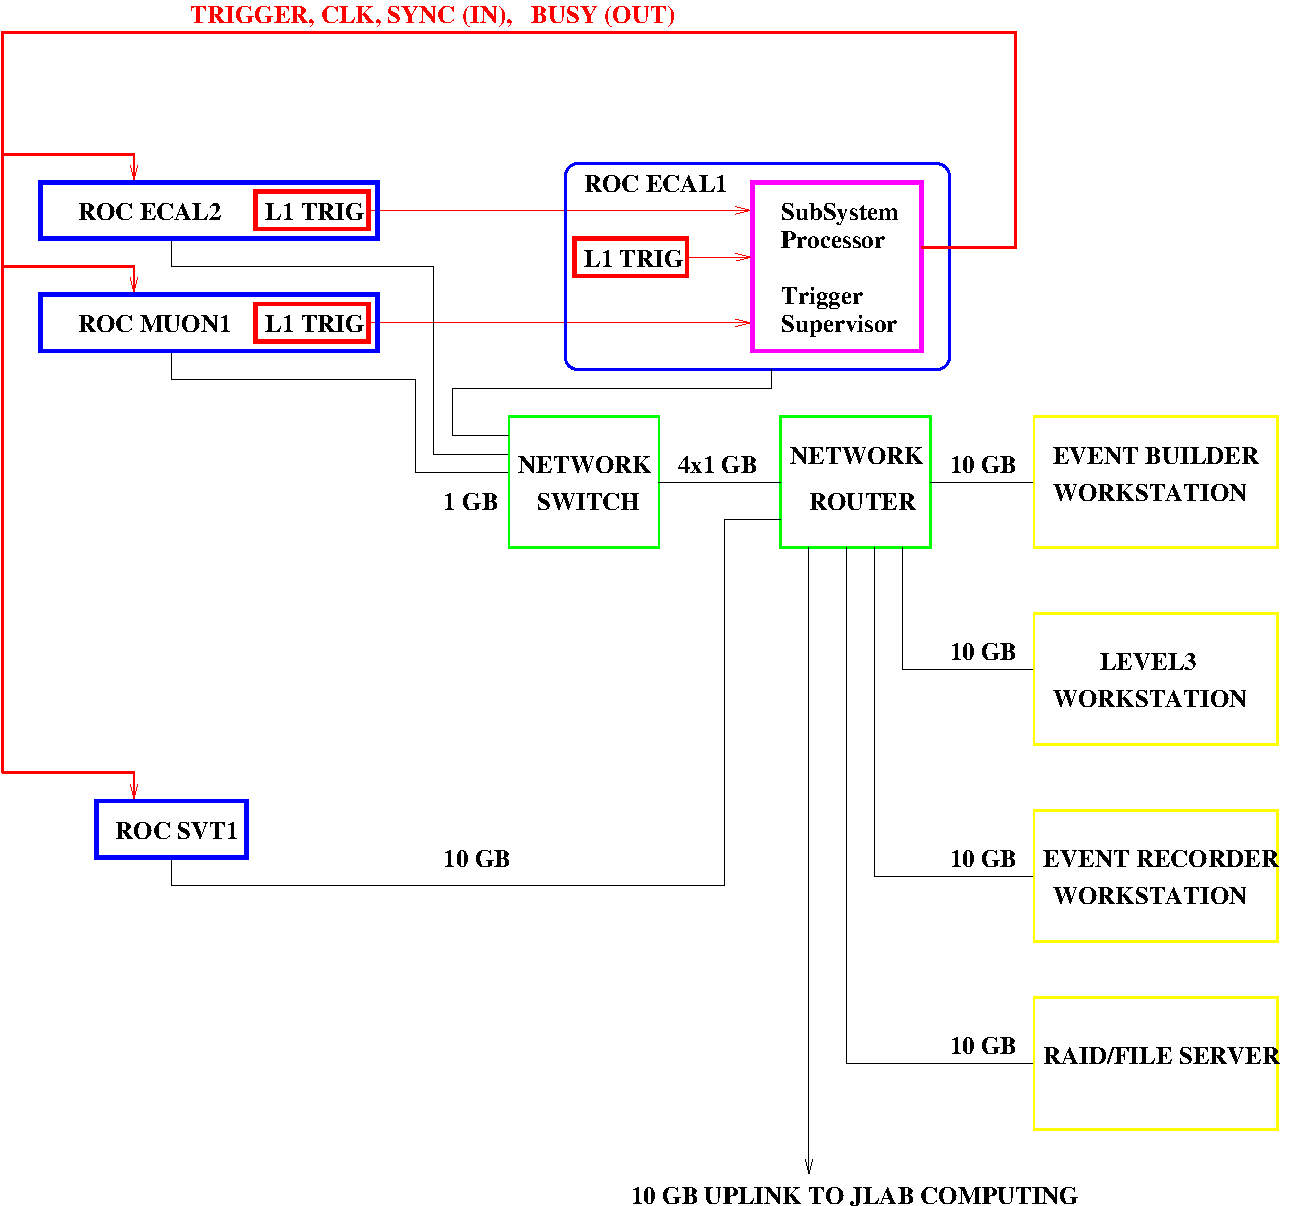
\includegraphics[ scale=0.7]{daq_trigger/figures/daq_schem.pdf}
\caption{\small{Schematic block diagram of the data acquisition system.}}
\label{fig:daq_hardware_overview}
\end{figure*}

For the ECal and Muon System, every VXS crate contains a Readout Controller (ROC) that collects digitized information, 
processes it, and sends it on to the
Event Builder. The ROC is a single blade Intel-based CPU module running DAQ software under CentOS Linux OS. 
For the SVT ATCA system, the ROC application runs on an embedded 
processor situated on the ATCA main board.
The Event Builder assembles 
information from the SVT, ECal and Muon System ROCs into a single 
event which is passed to the Event Recorder that writes it to a data storage system capable of handling up to 100~MB/s.
The Event Builder and other 
critical components run on multicore Intel-based multi-CPU servers. The DAQ network system is a 
Foundry router providing high-speed connections between the DAQ components and 
to the JLab computing facility. The SVT ROC, which must handle large data volumes, has a 10~Gbit/s link to the Foundry router, while a 1~Gbit/s link is adequate for the ECal and Muon System. A 10~Gbit/s uplink to the JLab computing facility is used for long-term storage.

Section~\ref{sec:svt_daq} describes the SVT DAQ in more detail while the VXS based readout for 
the ECal and muon detector is described in Sec.~\ref{sec:fadc_daq}. The trigger 
system is explained in more detail in Sec.~\ref{sec:triggerdaq}.

\subsubsection{SVT Data Acquisition}
\label{sec:svt_daq}
The goal of the SVT DAQ is to support the continuous 40~MHz readout and processing of signals from 
the 36 silicon strip sensors of the SVT. I also selects and transfers those events that were identified by the 
trigger system to the JLab DAQ for further event processing at rates 
close to 50~kHz. High data volumes result from high occupancy in the detector, pile-up from multiple bunches,
and sampling pulse heights in six consecutive time buckets for each hit in order to facilitate 
reconstruction of the hit time to high accuracy.

The system adopted is an evolution of the SVT DAQ used for the HPS Test Run, described in 
Sec.~\ref{sec:testrun_daq}. Several features changed in
response to the new SVT design and the evolution of SLAC's ATCA system. The new SVT has nearly twice 
the number of sensors as the Test Run detector, 
necessitating a more compact way to transfer data and power to the individual sensor modules through the
vacuum flanges. Accordingly, the new system incorporates a front end board within the vacuum volume for 
power distribution and signal digitization,
allowing many fewer vacuum connections per sensor and less interference within the vacuum volume. 
Problems encountered with reflections on long twisted pair
data lines, although ultimately overcome, have been avoided altogether by incorporating a flange board just 
outside of the vacuum and adopting an optical link. The ATCA system has evolved to using optical input, so 
this change lets HPS optimally piggyback on SLAC's ATCA system development.  

Each of the 36 silicon strip sensors is connected to a 
hybrid board incorporating five 128-channel APV25 front-end 
ASICs~\cite{Jones:1069892,Raymond:2002yr}, see Figure~\ref{fig:hybrid_and_apv25_testrun}.
The APV25 ASIC, initially developed for the Compact Muon Solenoid silicon tracker  at the Large Hadron 
Collider at CERN, was chosen because it provides excellent signal to noise, analog output for optimal 
spatial resolution, and multi-bucket output for good time resolution. 
Each hybrid board has five analog output lines (one for each of the APV25 ASICs) which are sent to the  
front-end readout board using low power LVDS differential current signals over about 1~m of flex cable.
At the readout board, a preamplifier scales the APV25 differential current output to match 
the range of a 14-bit Analog to Digital Converter (ADC). Each front-end board services four hybrids. 
The ADC operates at the system clock frequency of 41.667~MHz.
The digitized output from the front-end board is sent through compact 8-pair mini-SAS cables to 
the vacuum flanges to connect to the external DAQ which resides outside the vacuum chamber. 
The front-end readout board houses a FPGA and buffers to allow for the control of the 
distribution of clock, trigger and I$^{2}$C communication with the APV25 ASICs. 
To further simplify the services and minimize cabling that enter through the vacuum flanges, it contains 
linear regulators to distribute and regulate three low voltage power lines to the APV25 ASICs and
the high voltage bias. Figure~\ref{fig:svt_daq_flange_fe_boards} shows a schematics layout of the 
downstream readout chain of the SVT.
 \begin{figure*}[]
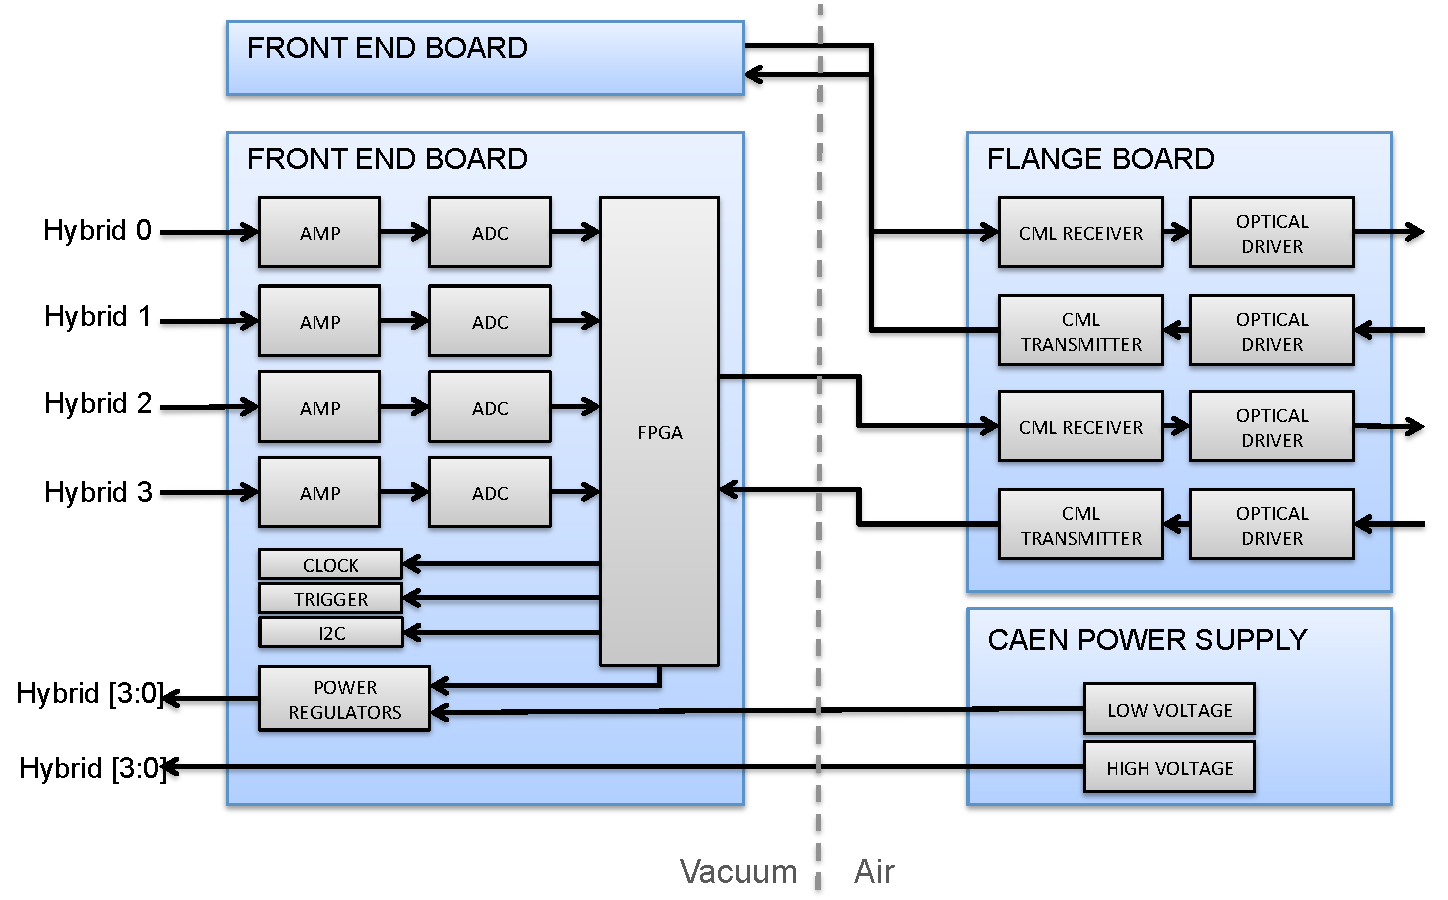
\includegraphics[ scale=0.6]{daq_trigger/figures/daq_hps_2014_schematics_fe_flange_boards.pdf} 
\caption{\small{Schematic overview of the front end and flange boards of the downstream part of 
SVT DAQ.}}
\label{fig:svt_daq_flange_fe_boards}
\end{figure*}

The digitized signals are converted to optical signals just outside the vacuum flange on custom built  
flange boards. Each flange board houses optical drivers to handle the electrical-optical 
conversion and to transmit the optical signals over $\sim 10$~m fibers to the SVT DAQ. 
The flange board also interfaces the low- and high voltage power transmission from the CAEN power 
supplies to the vacuum chamber.  

The main SVT DAQ uses the ATCA system for high speed data transfer. The optical signals from four hybrids, 
one half flange board, are received at one of four sections of the Rear Transition Module (RTM) boards of the 
ATCA crate, see Fig.~\ref{fig:svt_daq_overview}.
\begin{figure*}[]
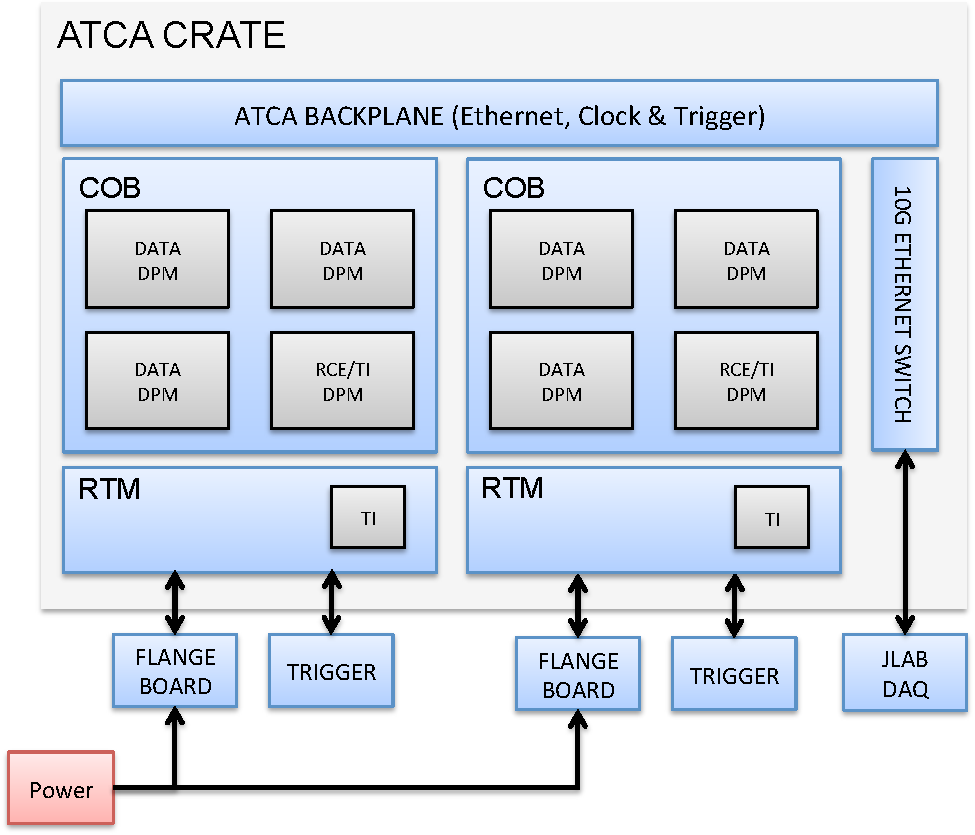
\includegraphics[ scale=0.6]{daq_trigger/figures/daq_hps_2014_schematics_atca.pdf} 
\caption{\small{Schematic block diagrams of the SVT data acquisition system.}}
\label{fig:svt_daq_overview}
\end{figure*}
Each section of the RTM connects to one of four FPGA units on the main ATCA board, 
the COB (Cluster On Board). Each FPGA is housed on a 
separate daughter board called a Data Processing Module (DPM). The modular ATCA design permits the 
HPS DAQ to re-use architecture and functionality from other DAQ system such as the ATLAS muon 
system which components are similar to that used by HPS. Figure~\ref{fig:rtm_testrun} shows the boards designed and used for the HPS Test run.
In order to minimize the complexity of the system inside the vacuum chamber, all signal processing is 
done at the DPM.  Each DPM receives the digitized signals 
from the RTM, applies thresholds for data reduction and organizes the sample data 
into UDP datagrams. One of the DPMs functions as the trigger interface which receives trigger 
signals from the optical fiber module on the RTM, distributes clock and trigger signals, 
and handles communication with the JLab trigger supervisor and the RCE. The 
RCE (Reconfigurable Cluster Element) is a generic computational building block 
on the trigger interface DPM running a 450~MHz PPC processor with 2~GB of DDR3 
memory. Four COBs housed in a two ATCA crates is sufficient to handle 
the 36 hybrids of the SVT.

The RCE receives and buffers UDP datagrams from the data and trigger DPMs and
 assembles them into full event frames. The RCE also runs an implementation of the JLab ROC application 
that integrates the SVT event frames into the JLab DAQ 
 system described above. The RCE node transfers data to the JLab DAQ  
 through a 10~Gbit/s Ethernet backend interface. The maximum readout rate of the SVT is approximately 50~kHz, limited by the APV25 readout rate. 
%The maximum readout rate of the SVT DAQ  is limited by the readout time 
%of the APV25 chip. Using overlapping trigger and readout functionality, where the 
%APV25 chip can buffer up to 5 triggers, the maximum average readout rate expected for 
%HPS is 45kHz {\color{red} need verification}.   










\subsubsection{ECal and Muon Detector FADC Readout}
\label{sec:fadc_daq}
The readout of the ECal and Muon System are essentially identical. 
The analog signals from the individual APD's of the ECal (shaped and amplified as described in Sec.~\ref{sec:ecal}) and phototubes of the Muon System are input to a single channel on the 16-channel JLab FADC250 VXS module (FADC), shown in Fig. ~\ref{fig:fadc}. 

Three 20-slot VXS crates needed to accommodate the system: one for each half of the ECal with 221 channels and one for the muon detector with a total of 232 channels.

\begin{figure}[t]
\includegraphics[scale=0.5]{daq_trigger/figures/FADC250_Photo_001.jpg}
\caption{\small{A Jefferson Lab FADC250 VXS module.}}
\label{fig:fadc}
\end{figure}

The FADC store 12-bit digitized samples at 250~MHz in 8~$\mu$s deep pipelines. 
When a trigger is received, the appropriate part of the pipeline is accessed. If a FADC   
signal exceeds a predefined threshold within that time window, the integrated amplitude of a pre-defined  number of samples before (NSB) and after (NSA) the signal passed threshold in addition to the time are recorded as explained in Fig.~\ref{fig:hps_trigger_data}. This scheme significantly compresses the data input to the FADC. During data analysis, a pedestal value is subtracted to obtain the actual summed energy.

%% Step %% The FADCs are an integral part of the HPS calorimeter trigger system. Energies  and times from each FADC channel in the same VXS crate are input to the crate trigger processor board (CTP) which groups adjacent channels with energy deposited into ``clusters,'' identifies the associated channels, andassigns an overall cluster energy. Clusters  from each CTP (one for the top half of the Ecal, one for the bottom) are combined in the sub-system processor module (SSP) which applies further selection criteria. Events with cluster combinations which pass the criteria are passed to the trigger supervisor. The trigger process has a pulse timing resolution of 4~ns. This allows a narrow coincidence window of 8~ns to be used when searching for clusters, and reduces accidental and out of time coincidences in the Ecal and the other systems. 

The main characteristics of the FADC are:
\begin{itemize}
\item 12-bit digitizer with sampling rate of 250~Msps, 
\item 50$\Omega$ termination input, 
\item front-end input range:  -0.5V, -1V or -2V (sufficient to avoid signal clipping for large pulse heights),
\item nominal charge resolution between 10-39~fC per ADC (see Tab.~\ref{tab:charge_resolution}).
\end{itemize}
\begin{table}[h]
\centering
\begin{tabular}{|c|c|}
\hline
Input range & Nominal charge resolution\\
(V) & (fC per ADC count)\\\hline
-0.5 & 9.76  \\\hline
-1.0 & 19.53  \\\hline
-2.0 & 39.06 \\\hline
\end{tabular}
\caption{Nominal FADC charge resolution for different front-end input ranges.}
\label{tab:charge_resolution}
\end{table}
The FADC will be operated in two modes, see Fig.~\ref{fig:hps_trigger_data}, that have different data paths:  the readout and trigger mode. 
In readout mode, every FADC have the following parameters:
 \begin{itemize}
 \item the number of samples integrated before the signal crossed threshold (NSB), 
 \item the number of samples integrated after the signal crossed threshold (NSA),
 \item the readout threshold, measured in ADC counts.
 \end{itemize}
The number of samples for a given channel integration is the sum of NSB+NSA samples. It is a fixed gate width pulse integration with no pedestal subtraction where the sum is stored in a 17-bit register for readout (pedestal subtraction happens offline). 
\begin{figure}[t]
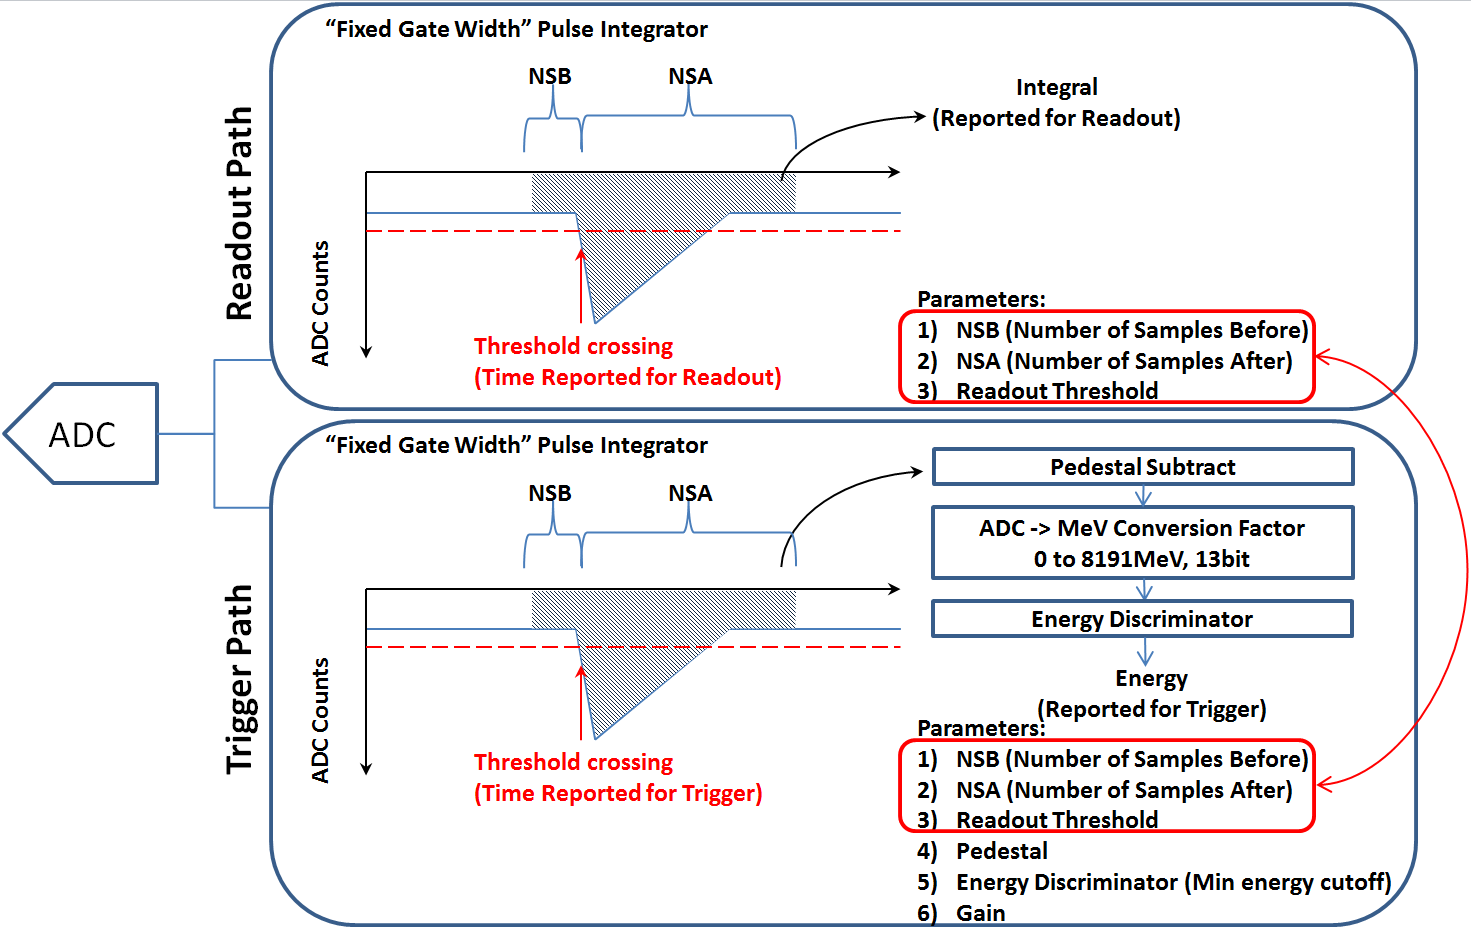
\includegraphics[scale=0.4]{daq_trigger/figures/hps_trigger_data}
\caption{\small{FADC data paths}}
\label{fig:hps_trigger_data}
\end{figure}

In the trigger mode, every channel has, in addition to the NSB, NSA and the threshold for the readout mode:  \begin{itemize}
% \item number of samples integrated before the threshold crossing (NSB),
 %\item number of samples integrated after the  threshold crossing (NSA),
 %\item trigger threshold, measured in ADC counts, 
 \item a pedestal, 
 \item a conversion factor (gain) that converts the ADC counts to energy in MeV (with 13 bits:  from 0 to 8191~MeV), 
 \item an energy discriminator threshold.
 \end{itemize}
Note that the threshold for the trigger mode can be set independently from the threshold used in readout mode.
The pedestal value is subtracted from the integrated sum over NSB+NSA samples and 
converted to MeV units using supplied gain conversion factor. The energy discriminator can be used to cut off low energy pulses before reporting to the Crate Trigger Processor (CTP). 
The values reported to the CTP are the 13-bit pulse energy and the time at which the pulse crossed the threshold. 
Data for every channel is sent to the CTP every 32~ns (if there is no hit a 0 energy pulse is sent) which sets a worst case double pulse resolution of 32~ns for individual channels, but less if pulses occur in adjacent 32ns windows.

%See Sec.~\ref{sec:triggerdaq} below for more details on the operation of the trigger system.






\subsubsection{Trigger System}
\label{sec:triggerdaq}

%\subsubsection{ECal Trigger overview}


The proposed trigger system is nearly deadtimeless. The trigger decision goes to the Trigger Supervisor every 4 ns. The trigger supervisor can apply deadtime if necessary, for example on a 'busy' or 'full' condition from front-end electronics.


\begin{figure}[t]
\includegraphics[scale=0.5]{daq_trigger/figures/FADC250_Photo_001.jpg}
\caption{\small{Jefferson Lab FADC250 VXS module.}}
\label{fig:fadc}
\end{figure}

The information from top and bottom parts of the ECal will be sent to the Jefferson Lab FADCs (Flash Analog-to-Digital Converters), Fig.~\ref{fig:fadc},  located in two different VXS crates (see Fig.~\ref{fig:hps_trigger_cal}). FADC  works at the frequency 250~MHz; i.e. it measures the amplitude of each ECal channel every 4 ns. FADC has 12bit pulse digitizer for readout and trigger processing. 

The first stage components of the trigger logic are incorporated into the Flash ADC board's FPGAs, while the final decision is made in a Crate Trigger Processors (CTPs) and  Sub-System Processor (SSP) .
FADC sends the information about the pulse energy and time to CTP.


\begin{figure}[t]
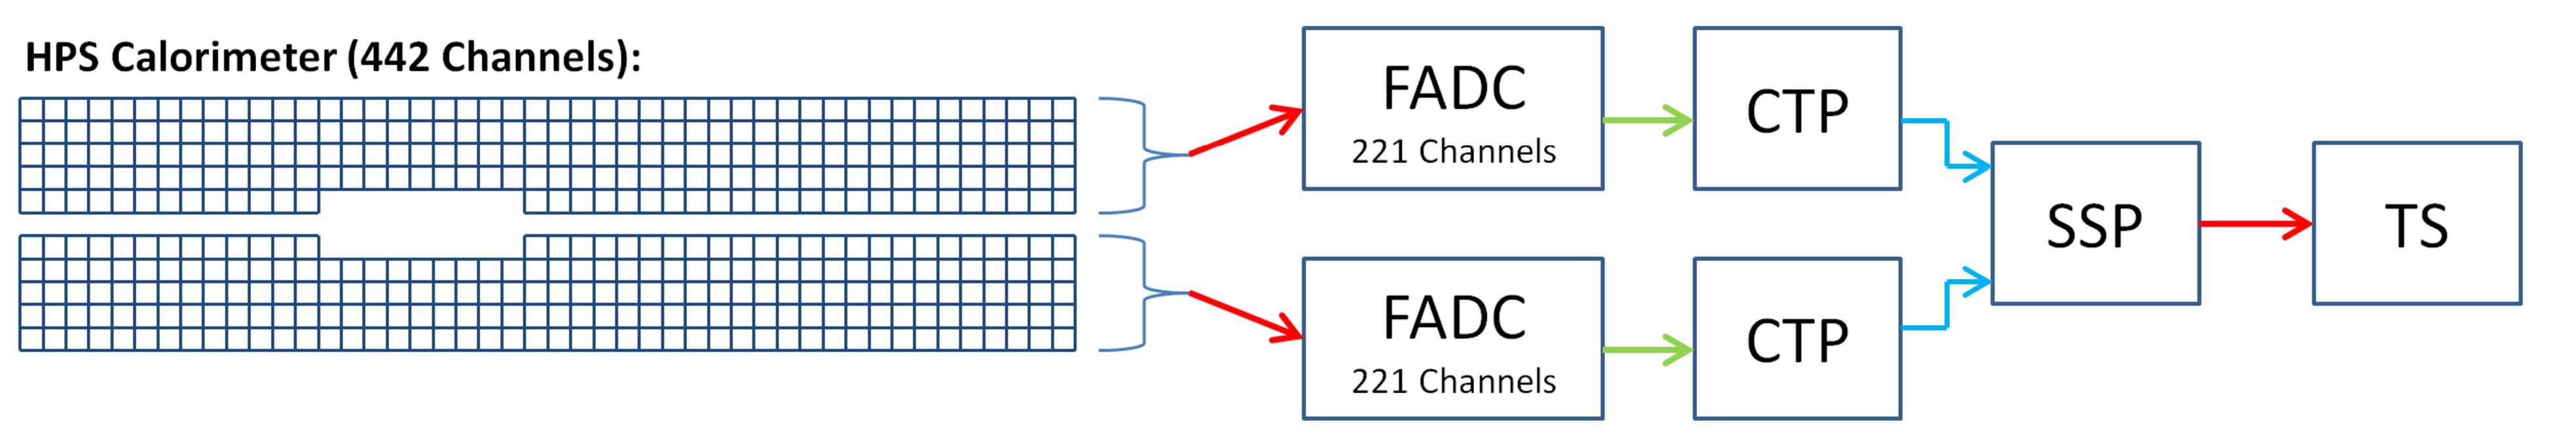
\includegraphics[scale=0.25]{daq_trigger/figures/hps_trigger_cal}
\caption{\small{ECAL trigger logic. FADC - Jlab Flash ADC, CTP - Crate Trigger Processor, SSP - Sub-System Processor, TS - Trigger Superviser.}}
\label{fig:hps_trigger_cal}
\end{figure}

The trigger system can be broken down into the following 3 sections:
 \begin{itemize}
 \item FADC (pulse finding): Samples the detector channel to find pulses. Pulse energy and times are sent to CTP.
 \item CTP (cluster finding): Searches FADC pulses (from half of calorimeter) to find clusters. Cluster energy, time, and hit pattern sent to SSP.
 \item SSP (cluster pair finding): Searches CTP clusters (from top and bottom) to find cluster pairs and create the trigger. Trigger cuts on pairs decide final trigger.
 \end{itemize}
 
 Trigger logic will search for a time coincidence between two clusters in opposite halves of ECal that occur within a programmable time window with 4ns resolution. The maximum trigger decision time (latency) is currently set to 3 $\mu$s for Level 1. That value is defined by the SVT readout APV25 chip.

The Trigger Supervisor generates all necessary signals, and controls the entire DAQ system readout through the Trigger Interface units. The Trigger Interface (TI) units installed in every crate participate in the readout process. The system is free-running and driven by a 250MHz global clock. The maximum trigger accept rate is 50 KHz.



%\subsubsection{Crate Trigger Processor} 

The Crate Trigger Processor receives the energy pulses (in MeV) and time stamp from each FADC channel in the crate (see Fig.~\ref{fig:hps_trigger_3x3}).
The algorithm used for cluster finding makes use the parallel processing nature of FPGAs by simultaneously searching for 125 clusters up to 3x3 in size across the calorimeter crystal array.  
A Cluster Processor (CP) algorithm:

\begin{itemize}
\item Add energy from hits together for every 3x3 square of channels in ECal
\item Hits are added together if they occur (leading edge) within a programmable number of clock cycles of each other (4 ns steps)
\item If 3x3 energy sum $\ge$  the programmable cluster energy threshold CTP reports cluster to the Sub-System processor the cluster parameters (time, energy, position and 3x3 hit pattern. 
\end{itemize}

Every 4ns the CTP evaluates all hits in its half of the calorimeter. A programmable time window is used to allow hits that are out of time with each other be considered as part of a cluster sum. This is done by reporting hits when they occur and then reporting them again for the next N number of 4 ns clock period, where N can be 0 to 7. This is useful to deal with skew and jitter that develop from the detector, cabling, and electronics.

When the sum of all hits in the 3x3 window occurring in a programmable time window are greater than the programmable energy threshold the cluster processor will report this cluster to the SSP if the energy is greater than all neighboring (up, down, left, right, and diagonals) 3x3 window cluster energies for that clock cycle. If the energy is not greater than its neighbor it will not be reported, but the neighbor will report if it is the greatest. The reason for this filtering is because there are several 3x3 windows that overlap and see the sample crystals and also many physics single clusters are larger than a 3x3 window.

The reported clusters to the SSP contain:

\begin{itemize}
\item 13bit Cluster energy (MeV)
\item Cluster position (crystal index: x,y)
\item Cluster time (4ns resolution)
\item Cluster hit pattern 3x3 (detector channels reporting a hit in the cluster)
\end{itemize}

The cluster position is the coordinate of the cluster processor that reported the cluster, which is where the peak cluster energy was seen from a 3x3 view. The 3x3 cluster hit pattern can be used by the SSP to help filter strange cluster patterns and/or make a low resolution cluster centroid computation.

\begin{figure}[h]
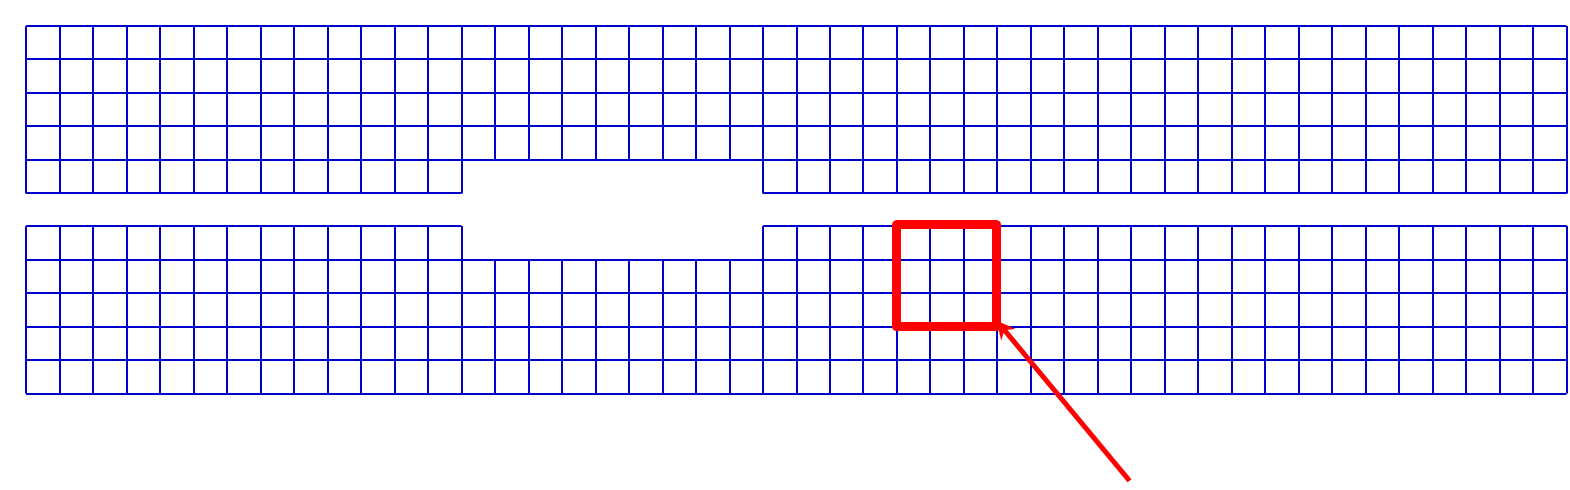
\includegraphics[scale=0.4]{daq_trigger/figures/hps_trigger_3x3}
\caption{\small{Cluster finding algorithm.}}
\label{fig:hps_trigger_3x3}
\end{figure}




%\subsubsection{Sub-System Processor} 

The cluster's time, energy, position and 3x3 pattern found in two VXS crates are reported to the Sub-System Processor. 
The SSP collects the cluster information from the full calorimeter and can create the trigger decisions of two types:
single cluster trigger and multi-cluster triggers.
Single cluster trigger condition includes the check on the cluster energy, $E_{min}\le E_{cluster}\le E_{max}$, where $E_{min}$ and $E_{max}$ are programmable minimum and maximum cluster energy.

Pairs trigger includes more conditions
\begin{itemize}
\item Energy sum,  
$E_{min}\le E_{top}+E_{bottom}\le E_{max}$
\item Pair time coincidence, 
$|t_{top}-t_{bottom}|\le \Delta t_{max}$ 
\item Energy difference, 
$|E_{top}-E_{bottom}|\le \Delta E_{max}$ 
\item Energy slope,
$E_{cluster\_with\_min\_energy}+R_{cluster\_with\_min\_energy}\times F_{energy}\le Threshold_{slope}$
\item Co-planarity, 
$|
tan^{-1}(\frac{X_{top}}{Y_{top}})-
tan^{-1}(\frac{X_{bottom}}{Y_{bottom}}) |\le Coplanarity_{angle}$
\item Number of hits in 3x3 window, 
\#$hits_{3\times 3}\ge HitThreshold$
\end{itemize}
\noindent
where $ E_{max}$,  $\Delta t_{max}$, $ \Delta E_{max}$ , $Threshold_{slope}$, 
$F_{energy}$, $Coplanarity_{angle}$
and
$HitThreshold$ are programable parameters.


Online event analysis will be provided to be compared against trigger event data for immediate verification (on each trigger cut: cluster energies, positions, timing, energy slope, coplanarity and hit threshold). With identical ADC readout and trigger pulse processing and high energy resolution, very precise agreement can be expected between trigger and readout.





%\subsubsection{Diagnostic Tools}

The previous experience with the similar (but much more simpler) trigger system showed that diagnostic tools are necessary to make sure that the calorimeter and trigger electronics work as expected. 

Scalers will be implemented for every ECal channel. The example of this diagnostic tool is presented in Fig.~\ref{fig:dvcs_beam}
from the previous version of the calorimeter. Hot or dead channels are easily identified online.
\begin{figure}[h]
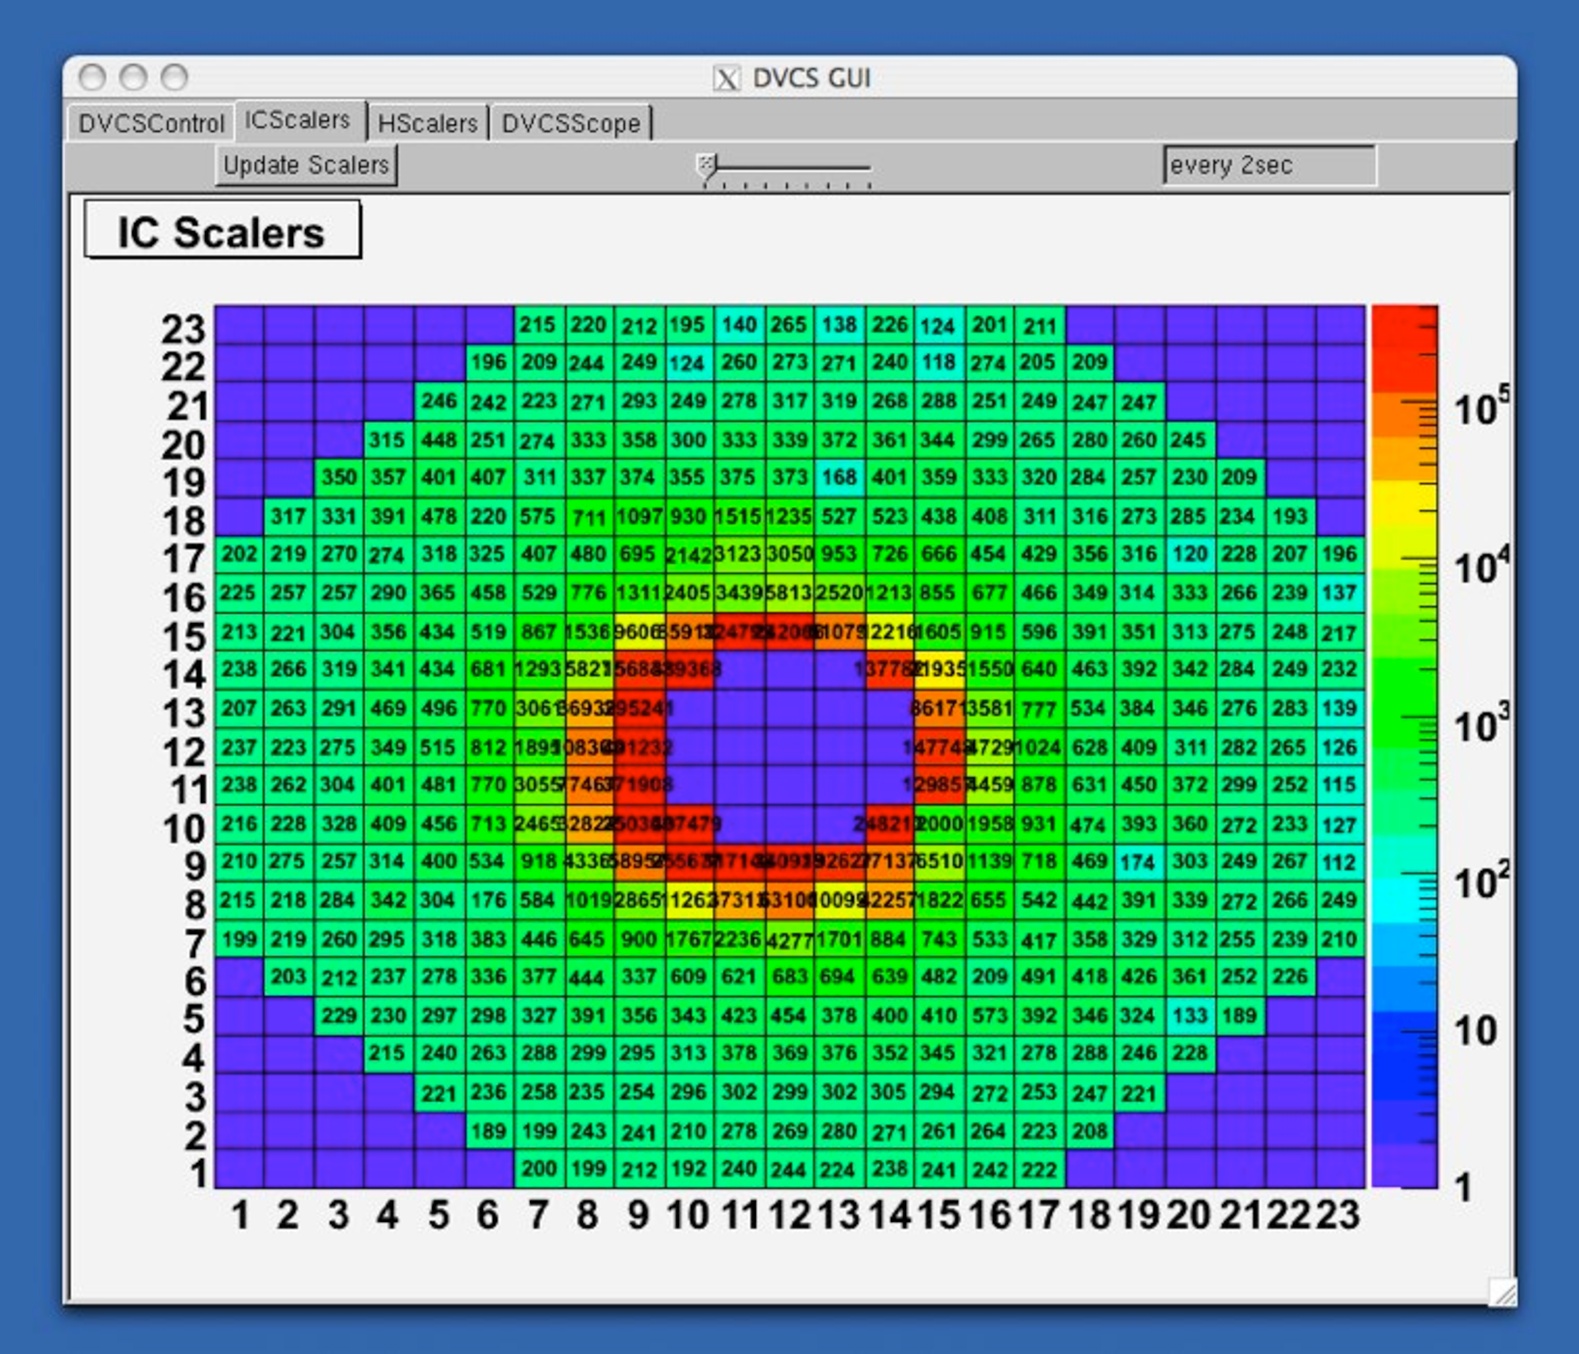
\includegraphics[scale=0.6]{daq_trigger/figures/dvcs_beam}
\caption{\small{Scalers (example from the previous version of the calorimeter).}}
\label{fig:dvcs_beam}
\end{figure}
Diagnostic scope permits to analyze on-line  the trigger logic. The goal to have  the Two-Dimensional Analyzer
 is to provide a remote debug interface to identify bad channels, verify cluster finding algorithms and check timing.
 The details of this analyzer are as following:
 
\begin{itemize}
\item Logic analyzer runs in parallel, non-intrusive, to the calorimeter trigger
\item Can setup trigger on any ECal pixel arrangement and/or cluster count
\item Can move forward/backward in time by ~250 ns to see timing details
\item Will be customize for HPS geometry and hardware
\end{itemize}

The example of the 2D analyzer is presented in Fig.~\ref{fig:dvcs_2_cluster}. Two clusters are displayed
in the picture. The red color displays the hits in the calorimeter and  the center of clusters is displayed in yellow.

In addition to the scalers, the distributions on individual ADC channel pulse energy will be provided.
The cluster hits positions and energy from SSP processor will be histogrammed as well. Two histograms (accepted and rejected) will be provided for each trigger cut used in the trigger logic.



\begin{figure}[t]
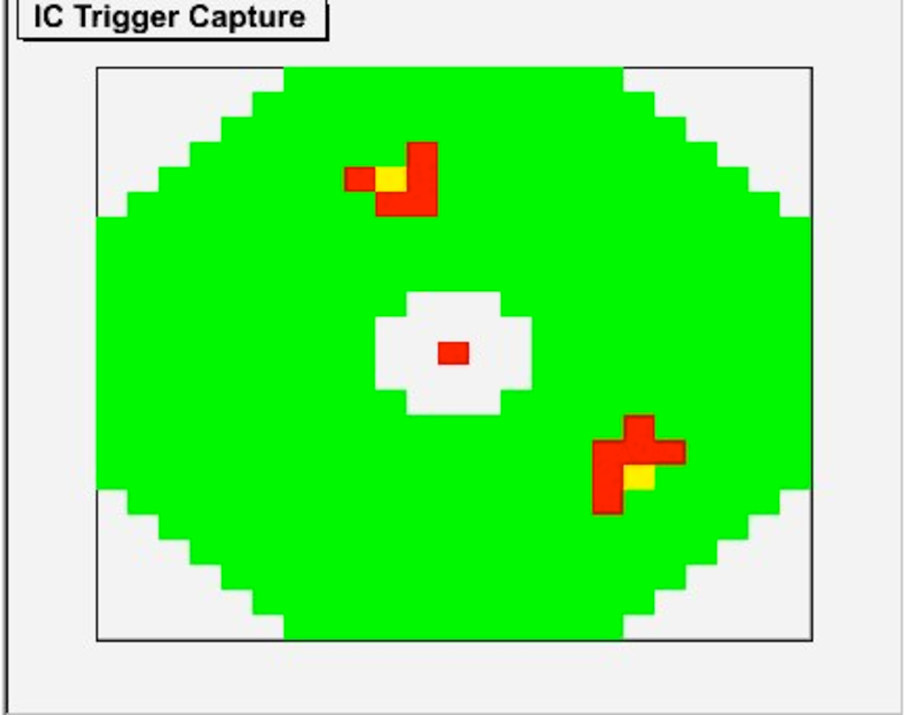
\includegraphics[scale=0.8]{daq_trigger/figures/dvcs_2_cluster}
\caption{\small{Diagnostic scope (example with two clusters found from the previous version of the calorimeter). Green - no hits, red - tower with hit, yellow - cluster found.}}
\label{fig:dvcs_2_cluster}
\end{figure}






%\subsubsection{Muon Trigger}

A muon detector composed of a four iron absorbers  and four double-layer scintillator planes, positioned after each absorber. Similar to the Ecal, the muon detector will consist of two halves, one above and one below the beam.
GEANT4 simulations have been used to study the trigger rates in the muon system due to background hits. It is expected that the true di-muon rate will be quite small compared to the ECal trigger rate and should not cause problem for the DAQ. 
A total of 144 readout channels are needed (9x16 channels multi-anode PMTs). Signals from each channel will be sent to a TDC and to a FADC. The FADC information will be used to construct the muon trigger. The TDC information together with information from FADC will be used in offline analysis to measure the hit position along the strip.

Selecting coincidence hits with MIP energy deposition in at least three layers of the scintillation hodoscope will identify muons. 
The muon trigger logic has to find one track in the top part of the detector in coincidence with another track in the bottom part of the detector. The track finding algorithm can be easily realized in the FPGA logic of the muon Crate Trigger processor.



\subsubsection{Event Size and Data Rates}

The high occupancies in the detector requires a high readout bandwidth to be able to transfer hits from the 
detectors to disk. The event sizes and rates are based on estimates from full Geant4-based simulations 
including all known backgrounds. As expected the SVT dominate the expected rates. 
The noise hit occupancy in the SVT is kept low by requiring that three of the six samples are above an
effective threshold of three times the noise level. The dominant contribution to the occupancy is instead 
the high rate of beam background hits estimated. This is estimated 
from detailed full simulation resulting in an occupancy of around 0.3\% or an average of 61 channels above threshold.  
%Background studies (see Sec.~\ref{sec:hps_perf}) show that 
%there are on average 10 tracks per event at a beam energy of 2.2~GeV and current of 
%200~nA. With each track 
%having on average 2 strips above threshold for each sensor there are on average 160 channels above threshold. Each of these channels will result in six digitized samples of the 
%pulse shape giving in total of 1084 samples per event for the SVT.
Each SVT channel has, in addition to the six digitized samples,  header information that identifies the 
the channel number and it's chip address. The complete SVT event size also 
include the overhead from each FPGA and the JLab data stream bank header.  
The maximum average event size increased with decreasing beam energy since a larger 
fraction of backgrounds get larger opening angles and thus potentially higher than the 15~mrad 
vertical dead zone angle. For a beam energy of 1.1~GeV, the average SVT event size is 2.5~kB and 
the rate is 43~MB/s, well within the SVT DAQ capabilities. 
The ECal and muon detectors, with occupancies between 3-10\%, each contribute with an event size of 
approximately 0.3~kB and maximum rates of about 12~MB/s for the 1.1~GeV run. 
%Each calorimeter or muon hit consist of 8 bytes (4 byte energy, 4 byte time)
 %with a 12 byte header (4 byte trigger number, 8 byte trigger time) for each FADC board. 
 Such rates are well within the 100~MB/s limit for each VXS crate used in the ECal and muon 
DAQ system.
 % for both the The main limitation is of the order of 100Mbytes/s from each VXS crate. For a 
% 10\% occupancy estimated in Sec.~\ref{sec:trig_rate} the ECal event size is approximately 0.7~kbytes which translates to a total data rate of approximately 31.5~Mbytes/s 
%(split between the two VXS crates), well within the DAQ system design. 
%The contribution from the muon system is small due to it's significantly lower number of channels. The system is readout by nine FADC boards in a single VXS crate. The event 
%size for a 10\% occupancy level is 0.2~kbytes which translates to a data rate of 10~Mbytes/s. 
Table~\ref{tab:data_rates} summarizes the event size and data rates. The highest overall rate, for a 1.1~GeV run, and that needs to be written to disk is 52~MB/s which is within the current 
DAQ system design limit of 100~MB/s. 
\begin{table}[]
\centering
\begin{tabular}{|l|ccc|ccc|ccc|}
\hline
 & \multicolumn{3}{|c|}{Occupancy(\%)} &  \multicolumn{3}{|c|}{Event size (kB)} &  \multicolumn{3}{|c|}{Data rate (MB/s)} \\
\hline
Beam energy (GeV) & 1.1 & 2.2 & 6.6 & 1.1 & 2.2 & 6.6 & 1.1 & 2.2 & 6.6 \\
\hline
SVT & 0.5 & 0.3  & 0.3  & 2.5 & 1.7 & 1.5 & 55.4 & 35.8 & 26.4\\
ECal & 3.0 & 4.2  & 4.7 & 0.3 & 0.3  & 0.3 & 6.3 & 6.3  & 5.5 \\
Muon & 10 &  10 & 10  & 0.2 & 0.2 & 0.2 & 4.9 & 4.5 & 3.8 \\
\hline
Total& \multicolumn{3}{|c|}{-} & 3.0 & 2.2 & 2.0 & 66.6 & 46.6 & 35.7 \\
\hline
\end{tabular}
\caption{{\small Summary of the occupancy, event size and data rate expected for the runs at  runs at the three beam 
energies in the run plan. }}
\label{tab:data_rates}
\end{table}
